%%% MATERIALS AND METHODS %%%


Put materials and methods used here.

\subsection*{Carbon Fiber Filament}

test text\\

\subsection*{Extruder Design}

test text\\

\subsection*{Finite Element Analysis}

ANSYS Composite PrepPost (ACP) finite element analysis software was used to predict the mechanical properties and failure behavior of the bridge specimen. ACP utilizes orthopic shell elements, ply thickness assignments, oriented element sets, and stackup configurations to model and analyze fiberous, composite structures of multiple layers. Various failure criteria, such as Puck or Tsai-Wu failure theories, are utilized in solving to predict failure modes and critical layers given the applied loads and boundary conditions.

\begin{figure}[htp]
%\centering
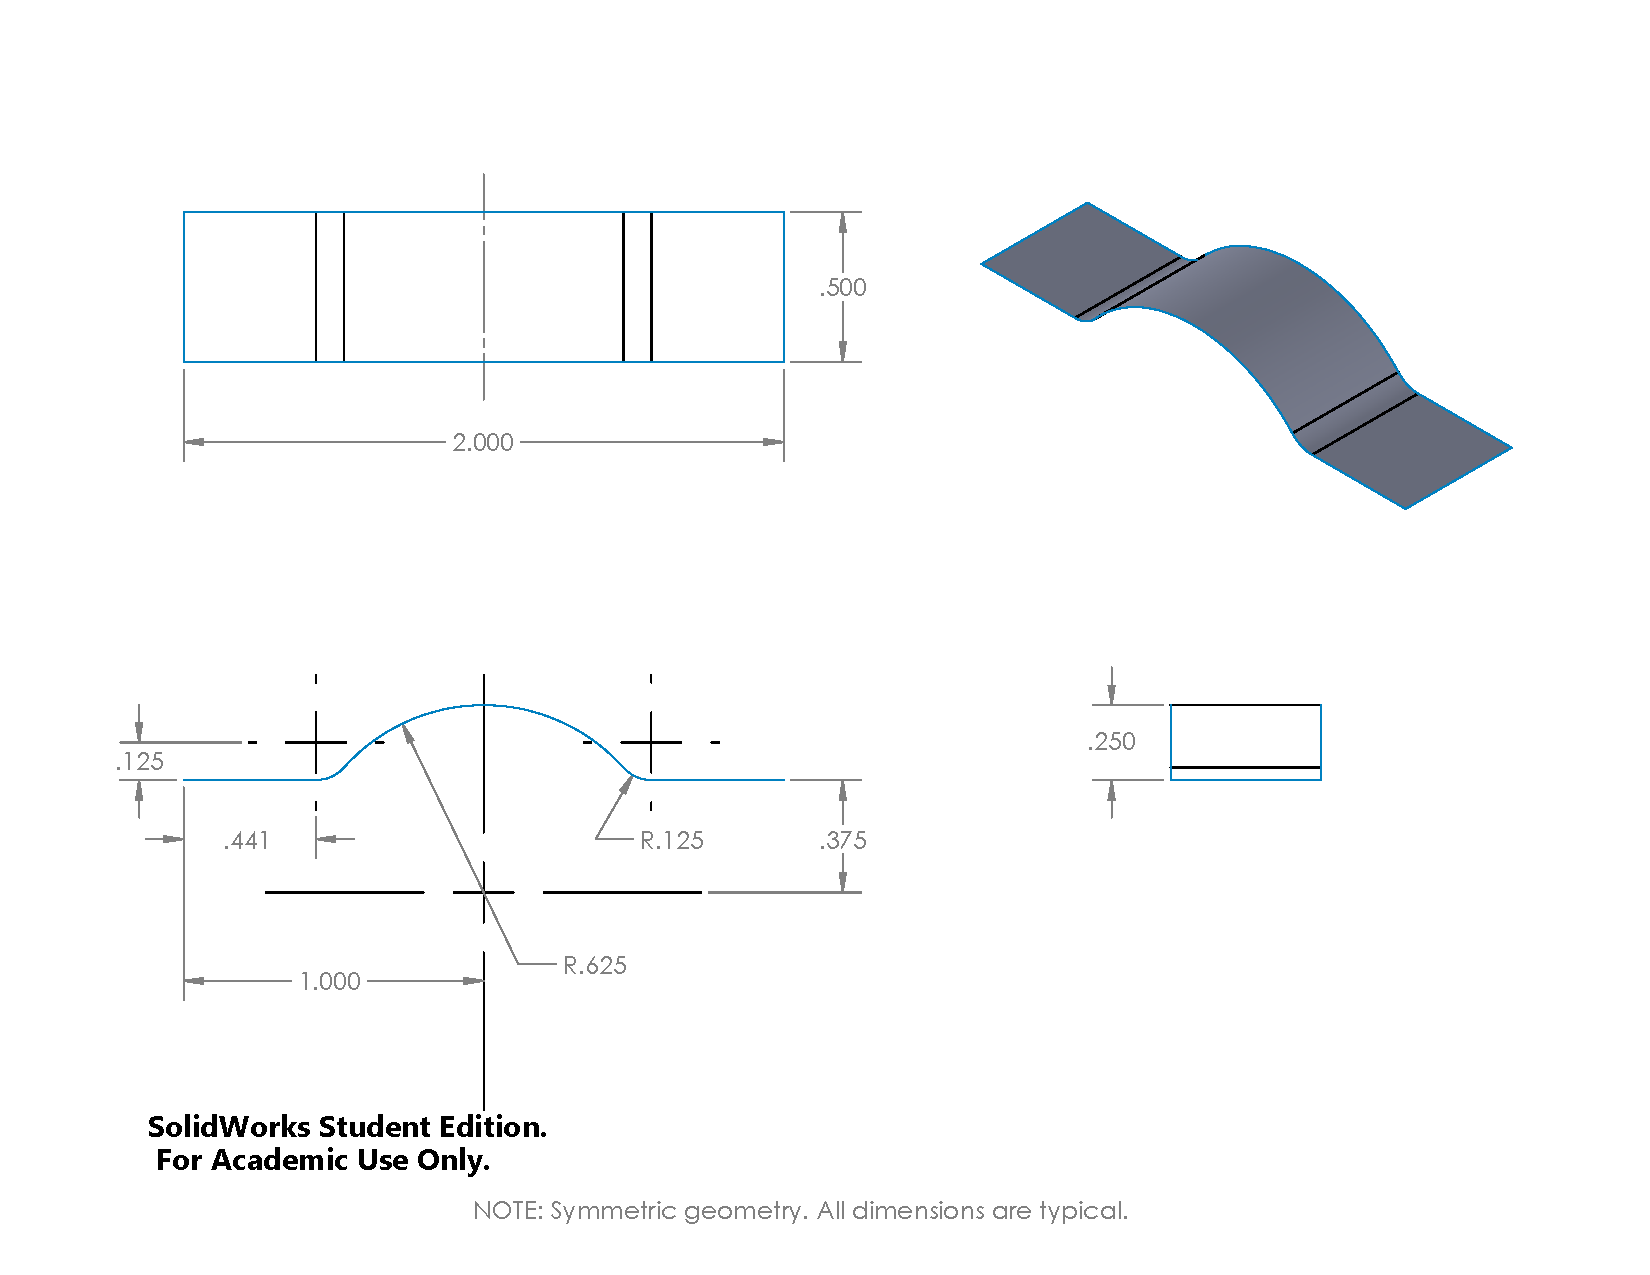
\includegraphics[width=0.4\textwidth]{./figures/fea/fea-surface-geometry}
\caption{The surface geometry used in ACP.}
\label{fig:fea-bridge-speciment}
\end{figure}

%test text. test citations \cite{Puck-Stuttgard,Puck-NASA}.\\

\subsection*{Print Controls}

test text\\

\subsection*{FANUC Setup}

test text\\